\asciicmd{curout?}{
    \index{user_cmds_index}{curout?}
    \label{cmd:curout}

    \textbf{Name:} \texttt{curout?} -- Query the output current.\\
    \textbf{Description:} Prints calibrated output current values in
    fixed-point $\mu$A to the remote interface.  As shown below,
    values are an average of the last four samples.  This represents
    an average over the last $4 \times \tau_c$ milliseconds.  See the
    \texttt{curper} command described \vpageref{cmd:curper} to set $\tau_c$.

    
    \begin{center}
        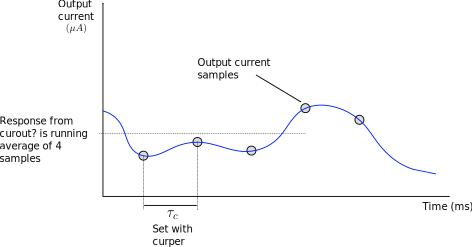
\includegraphics[clip,scale=0.9]{figs/curout_plot}
        \captionof{figure}{The value returned with the \texttt{curout?} query
        is an average of the last four output current samples.}
    \end{center}
 



    \textbf{Example:}
    \boxtext{\texttt{curout?}
      \codecomment{Query the output current}\\
      \texttt{7404}    \codecomment{Measured value is 7404$\mu$A}
    }

}